\subsubsection{Total number of collisions}\label{subsubsec:ld2krcollisions}

For the total number of collisions we get a very low unexplained variation
(\(0.64\%\)). The broadcast radius accounts for the \(58.96\%\) of the variation
and it is the dominant factor, as in the case of the high density scenario. In
the previous scenario, the second most important factor was the maximum relay
delay and the third was the maximum number of copies. Here, instead, we get that
the maximum number of copies accounts for the \(19.26\%\) of the variation while
the maximum relay delay accounts only for the \(7.37\%\) of the variation. In
this case, also the combination of the broadcast radius and the maximum number
of copies is relevant (\(9.65\%\)).

As in the case of the high density scenario, we need to decrease the broadcast
radius to reduce the total number of collision. As shown in
\figref{subfig:ldperfcollisionsm} using lower values for the maximum number of
copies reduces the total number of collisions, as expected.
\figref{subfig:ldperfcollisionsD} shows that an higher value for \(D\) means
a lower number of collisions.

The fact that the broadcast radius is less important in this scenario compared
to the high density case can be explained by the fact that the users are more
scattered in the floorplan, so we need a huger increase of the broadcast radius
to see an effect.

\begin{figure}[htb]
	\centering
	\begin{subfigure}[b]{0.49\textwidth}
		\centering
		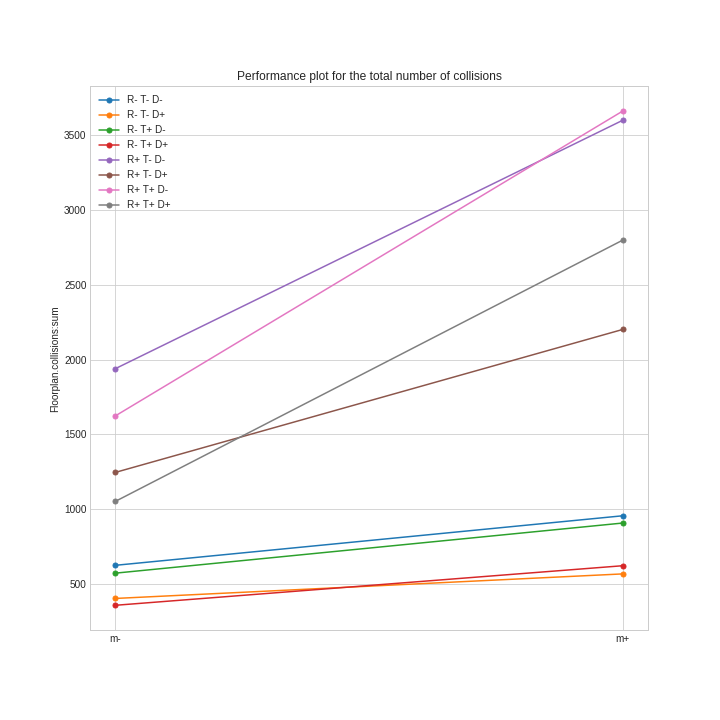
\includegraphics[width=\textwidth]{img/ld/collisions-m-perfplot}
		\caption{Decrease the maximum number of copies to decrease the
		total number of collisions}\label{subfig:ldperfcollisionsm}
	\end{subfigure}
	\begin{subfigure}[b]{0.49\textwidth}
		\centering
		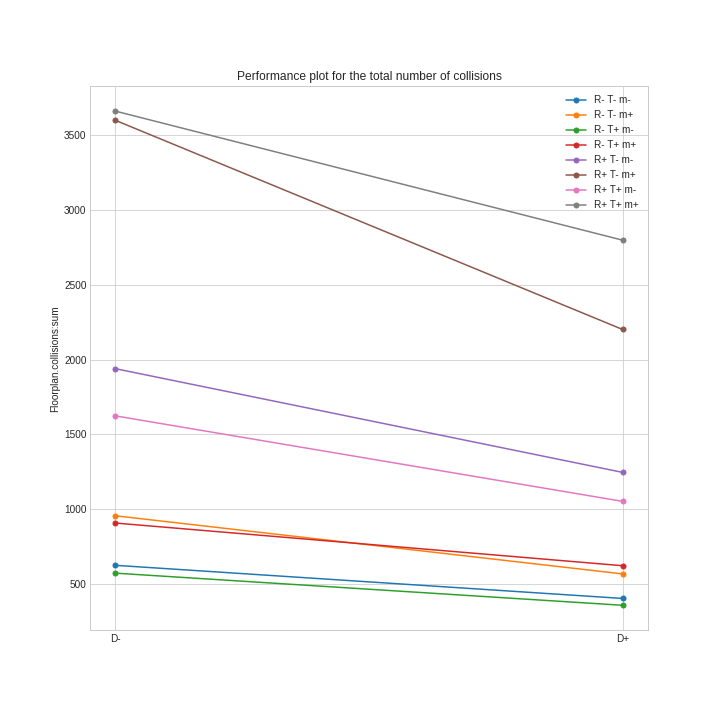
\includegraphics[width=\textwidth]{img/ld/collisions-D-perfplot}
		\caption{Increase the maximum relay delay to reduce the total
		number of collisions}\label{subfig:ldperfcollisionsD}
	\end{subfigure}
	\caption{Performance plots for the total number of
	collisions}\label{fig:ldperfcollisions}
\end{figure}
